\documentclass{article}

\usepackage{fancyhdr}
\usepackage{extramarks}
\usepackage{amsmath}
\usepackage{amsthm}
\usepackage{amsfonts}
\usepackage{tikz}
\usepackage{algpseudocode}
\usepackage{caption}
\usepackage{subcaption}
\usepackage{listings}
\usepackage{color}


\usetikzlibrary{automata,positioning}

%
% Basic Document Settings
%

% Custom sectioning
%\usepackage{sectsty}
%\allsectionsfont{\centering \normalfont\scshape}

\captionsetup{justification=centering,
singlelinecheck=false
}
\graphicspath{ {required/} }

\topmargin=-0.45in
\evensidemargin=0in
\oddsidemargin=0in
\textwidth=6.5in
\textheight=9.0in
\headsep=0.25in

\linespread{1.1}

\pagestyle{fancy}
\lhead{\hmwkAuthorName}
\chead{\hmwkClass}
\rhead{\hmwkTitle}
\lfoot{\lastxmark}
\cfoot{\thepage}

\renewcommand\headrulewidth{0.4pt}
\renewcommand\footrulewidth{0.4pt}

\setlength\parindent{0pt}

%
% Create Problem Sections
%

\newcommand{\enterProblemHeader}[1]{
    \nobreak\extramarks{}{Problem \arabic{#1} continued on next page\ldots}\nobreak{}
    \nobreak\extramarks{Problem \arabic{#1} (continued)}{Problem \arabic{#1} continued on next page\ldots}\nobreak{}
}

\newcommand{\exitProblemHeader}[1]{
    \nobreak\extramarks{Problem \arabic{#1} (continued)}{Problem \arabic{#1} continued on next page\ldots}\nobreak{}
    \stepcounter{#1}
    \nobreak\extramarks{Problem \arabic{#1}}{}\nobreak{}
}

\setcounter{secnumdepth}{0}
\newcounter{partCounter}
\newcounter{homeworkProblemCounter}
\setcounter{homeworkProblemCounter}{1}
\nobreak\extramarks{Problem \arabic{homeworkProblemCounter}}{}\nobreak{}

%
% Homework Problem Environment
%
% This environment takes an optional argument. When given, it will adjust the
% problem counter. This is useful for when the problems given for your
% assignment aren't sequential. See the last 3 problems of this template for an
% example.
%
\newenvironment{homeworkProblem}[1][-1]{
    \ifnum#1>0
        \setcounter{homeworkProblemCounter}{#1}
    \fi
    \section{Problem \arabic{homeworkProblemCounter}}
    \setcounter{partCounter}{1}
    \enterProblemHeader{homeworkProblemCounter}
}{
    \exitProblemHeader{homeworkProblemCounter}
}

%
% Homework Details
%   - Title
%   - Due date
%   - Class
%   - Section/Time
%   - Instructor
%   - Author
%

\newcommand{\hmwkTitle}{Homework\ 5}
\newcommand{\hmwkDueDate}{February 20, 2015}
\newcommand{\hmwkClass}{Information Integration on the Web}
\newcommand{\hmwkClassInstructor}{Prof. Ambite \& Knoblock}
\newcommand{\hmwkAuthorName}{Tushar Tiwari}

%
% Title Page
%

\title{
    \vspace{2in}
    \textmd{\textbf{\hmwkClass:\ \hmwkTitle}}\\
    \normalsize\vspace{0.1in}\small{Due\ on\ \hmwkDueDate}\\
    \vspace{0.1in}\large{\textit{\hmwkClassInstructor}}
    \vspace{3in}
}

\author{\textbf{\hmwkAuthorName}}
\date{}

\renewcommand{\part}[1]{\textbf{\large Part \Alph{partCounter}}\stepcounter{partCounter}\\}

%
% Various Helper Commands
%

% Useful for algorithms
\newcommand{\alg}[1]{\textsc{\bfseries \footnotesize #1}}

% For derivatives
\newcommand{\deriv}[1]{\frac{\mathrm{d}}{\mathrm{d}x} (#1)}

% For partial derivatives
\newcommand{\pderiv}[2]{\frac{\partial}{\partial #1} (#2)}

% Integral dx
\newcommand{\dx}{\mathrm{d}x}

% Alias for the Solution section header
\newcommand{\solution}{\textbf{\Large Solution}}

% Probability commands: Expectation, Variance, Covariance, Bias
\newcommand{\E}{\mathrm{E}}
\newcommand{\Var}{\mathrm{Var}}
\newcommand{\Cov}{\mathrm{Cov}}
\newcommand{\Bias}{\mathrm{Bias}}

% Language Definitions for SPARQL
\definecolor{olivegreen}{rgb}{0.2,0.8,0.5}
\definecolor{grey}{rgb}{0.5,0.5,0.5}
\lstdefinelanguage{ttl}{
sensitive=true,
morecomment=[l][\color{grey}]{PREFIX},
morecomment=[l][\color{grey}]{BASE},
morecomment=[l][\color{olivegreen}]{SELECT},
morestring=[b][\color{blue}]",
showstringspaces=false,
}
\lstset{%
  numbers=none,
  tabsize=4,
  breaklines=true,
  basicstyle=\small\ttfamily,
  framerule=10pt,
  columns=fullflexible,
  language=ttl
}

\begin{document}

\maketitle

\pagebreak
\begin{homeworkProblem}
    {Briefly describe the selected fields}.\hfill [15 points]
    \begin{flushleft}
        \solution\\
        \subsection{display}
        The display field states the manner in which the painting is displayed. Whether it is displayed within a frame or just a canvas or a panel or just a sheet.\par
        \subsection{acquired\_id}
        The acquired\_id is a sort of transaction id for the acquisition of the painting.
        \subsection{acquired\_from}
        The acquired\_from is the description of from whom was the painting acquired and by what means.
        \subsection{artist2 - last,first name/link/birth year and death year}
        In the case when the painting has only one author then artist1 - (...) fields are filled in with artist2 - (...) fields empty. But if a painting has multiple authors then there are multiple rows for that many authors and the author2 - (...) fields are filled in and the author1 - (...) fields empty.
        \subsection{bibliography}
        Bibliography is the list of sections for the painting.
    \end{flushleft}
\end{homeworkProblem}
\pagebreak
\begin{homeworkProblem}
    {Explain the cleaning operations performed for each field}.\hfill [50 points]
    \begin{flushleft}
        \solution\\
        \subsection{display}
        The display field had values like framed, Framed, Frame and unspecified, (blank). So these values were combined. To combine these values first create a text facet on the display column. Then I manually edited in the facets. Changed Frame, framed to Framed and changed unspecified to (blank)
        \subsection{acquired\_from}
        The acquired\_from field was missing data due to a faulty pull of data. While scraping the data, to separate acquired\_id from acquired\_from a split on \lq(\rq was done. However that did not work out well as there was a \lq(\rq in the text of acquired\_from which was now copied into acquired\_id. So we basically had to strip acquired\_id of this text which belonged to acquired\_from and so we append the value of acquired\_id to acquired\_from.
        \begin{figure}[!ht]
            \centering
            \fbox{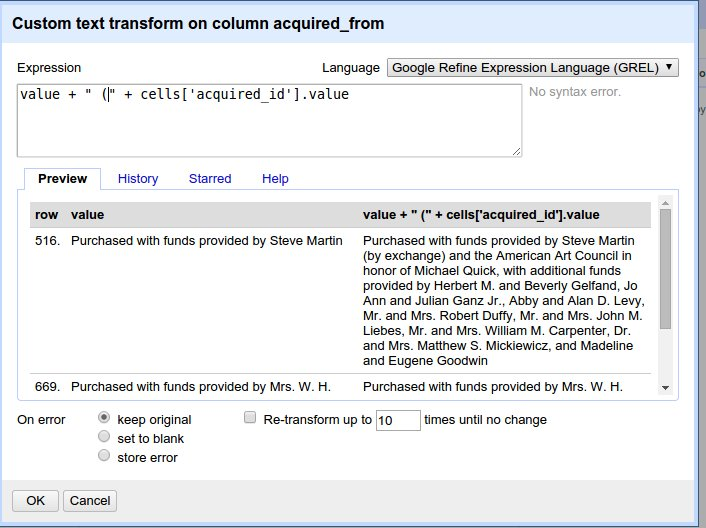
\includegraphics[width=0.95\textwidth]{clean_acquired_from}}
            \caption{Transform acquired\_from column}
        \end{figure}
        \pagebreak
        \subsection{acquired\_id}
        Since this data is not available for the rows whose acquired\_from was transformed previously(luckily only 2), we manually add the data.
        \subsection{artist2 - (...)}
        So these fields have been described before already. Quick note, after creating the project I have renamed all these columns from \_\_anonymous\_\_ - artist - \_\_anonymous\_\_ - (...) to artist2 - (...). Basically we want multiple rows of the painting for multiple authors which is already provided by openrefine while importing. Only problem the artist data exists in the artist2 fields. So all I have to do is copy every artist2 - (...) field to corresponding artist - (...) field. 
        \begin{itemize}
        \item I create a customized facet called facet by blank on artist - name - last and get all true records. That is, all records for whom artist - name - last is blank.
        \item Then on those records I create another customized blank facet on artist2 - name - last is false which fetched all records with some value other than blank for artist2 - name - last. Note that all records for which some value of artist2 exists artist will be blank by design.
        \item Now transform cells of artist - name - last by copying the artist2 - name - last.
        \item Repeat for all artist2 - (...) cells
        \item After copying all columns delete all the artist2 columns.
        \end{itemize}
        \begin{figure}[!ht]
            \centering
            \fbox{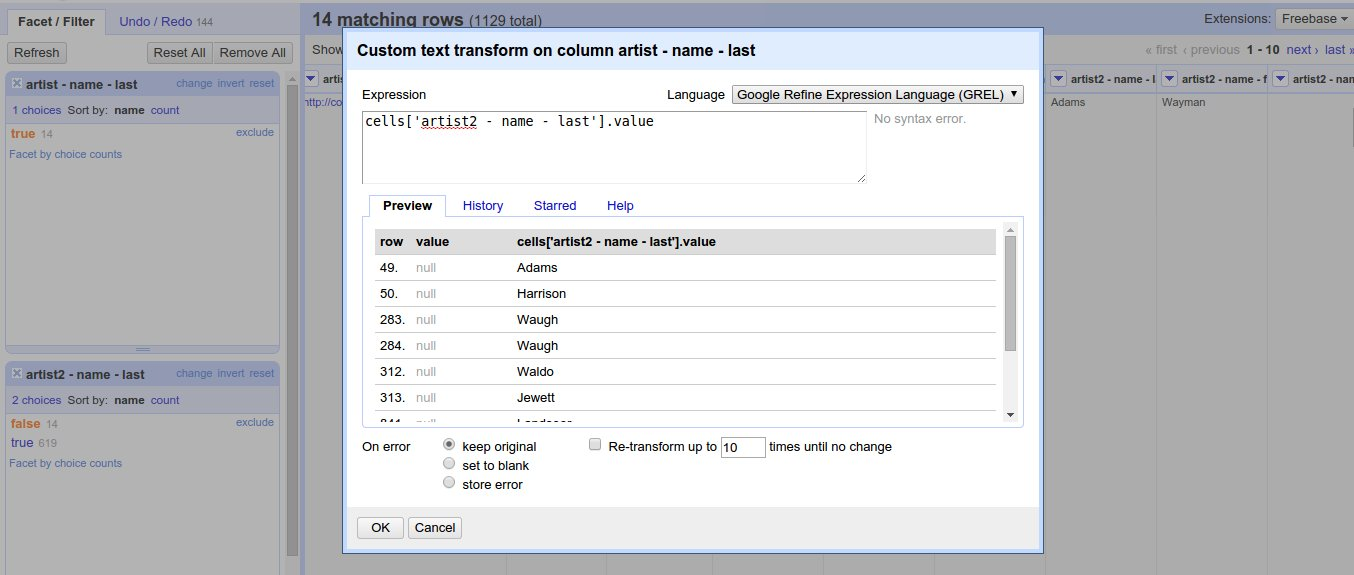
\includegraphics[width=0.95\textwidth]{clean_artist}}
            \caption{Transform artist - name - last column}
        \end{figure}
        \pagebreak
        \subsection{bibliography}
        For every item in the bibliography section of the painting, openrefine creates a new record for that painting. So we want to combine those different records that contain the different items of the bibliography section. To do this we shall
        \begin{itemize}
        \item Blank down on the link column if not already blank downed. If multiple records have similar links then only the topmost record will have the link. Make sure that the sort is on the links before blanking down.
        \item Move link column to beginning.
        \item Now in bibliography goto edit cells $>>$ Join multivalued cell. For the separator choose a unique separator such that a split can be performed at a later time on this data (I choose 'abcdefgh'). This action will push up and append all the different values of bibliography for that record into the topmost record and all lower records' bibliography value becomes null.
        \item All the extra rows created due to bibliography can be deleted because they will not contain any information for any column.
        \item Then do a secure fill down i.e. transform the column by doing row.record.cells["bibliography"].value[0]. This basically copies down the value of bibliography to same paintings only. A fill down will copy unless a new value is encountered.
        \item Finally transform the cell values by doing a forEachIndex(value.split('abcdefgh'), i ,val, (i+1) + ". " + val).join(" " ). This will nicely add a numbered ordering to the bibliography items.
        \end{itemize}
    \end{flushleft}
\end{homeworkProblem}
\pagebreak
\begin{homeworkProblem}
    {Show one example of the cleaning done for each field. Show the full record before and after cleaning.}.\hfill [15 points]
    \begin{flushleft}
        \solution\\
        \subsection{display}
        \begin{figure}[!ht]
        \centering
        \begin{subfigure}{0.4\textwidth}
        \centering
        \fbox{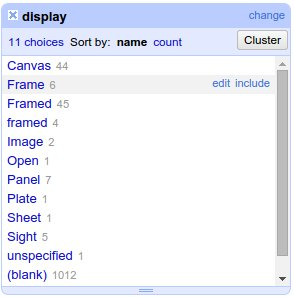
\includegraphics[width=0.95\textwidth]{clean_display_before1}}
        \caption{The facets}
        \end{subfigure}
        \begin{subfigure}{0.4\textwidth}
        \centering
        \fbox{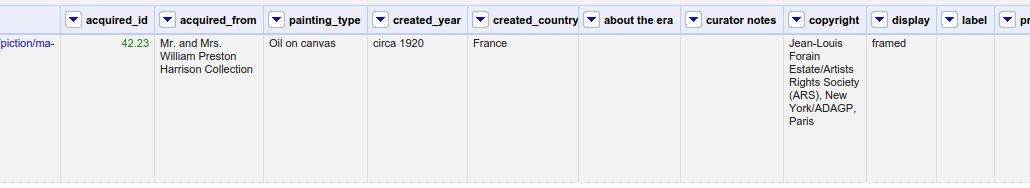
\includegraphics[width=0.95\textwidth]{clean_display_before2}}
        \caption{A record}
        \end{subfigure}
        \caption{Before cleaning display}
        \end{figure}
        \begin{figure}[!ht]
        \centering
        \begin{subfigure}{0.4\textwidth}
        \centering
        \fbox{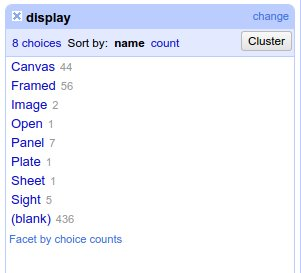
\includegraphics[width=0.95\textwidth]{clean_display_after1}}
        \caption{The facets}
        \end{subfigure}
        \begin{subfigure}{0.4\textwidth}
        \centering
        \fbox{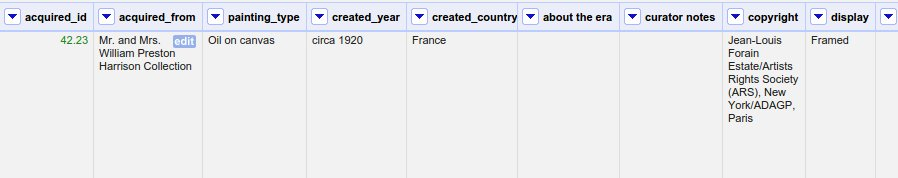
\includegraphics[width=0.95\textwidth]{clean_display_after2}}
        \caption{A record}
        \end{subfigure}
        \caption{After cleaning display}
        \end{figure}
        \pagebreak
        \subsection{acquired\_from \& acquired\_id}
        \begin{figure}[!ht]
        \centering
        \fbox{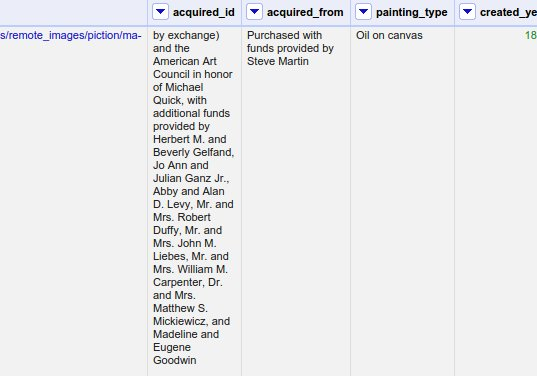
\includegraphics[width=0.8\textwidth]{clean_acquired_before}}
        \caption{Before cleaning}
        \end{figure}
        \begin{figure}[!ht]
        \centering
        \fbox{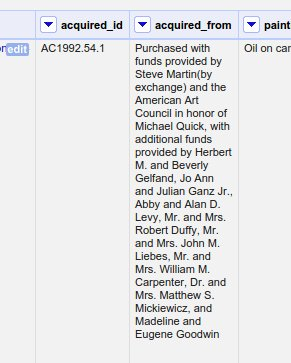
\includegraphics[width=0.4\textwidth]{clean_acquired_after}}
        \caption{After cleaning}
        \end{figure}
        \pagebreak
        \subsection{artist2 - (...)}
        \begin{figure}[!ht]
        \centering
        \begin{subfigure}{0.95\textwidth}
        \centering
        \fbox{
\includegraphics[width=0.95\textwidth]{artist2_before1}}
        \caption{1st artist of some painting}
        \end{subfigure}
        \begin{subfigure}{0.95\textwidth}
        \centering
        \fbox{
\includegraphics[width=0.95\textwidth]{artist2_before2}}
        \caption{2nd artist of same painting}
        \end{subfigure}
        \caption{Before cleaning}
        \end{figure}
        \begin{figure}[!ht]
        \centering
        \begin{subfigure}{0.95\textwidth}
        \centering
        \fbox{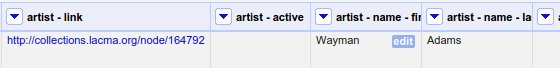
\includegraphics[width=0.95\textwidth]{artist2_after1}}
        \caption{1st artist of some painting}
        \end{subfigure}
        \begin{subfigure}{0.95\textwidth}
        \centering
        \fbox{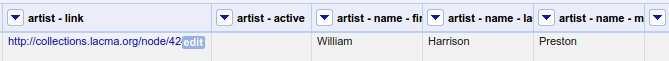
\includegraphics[width=0.95\textwidth]{artist2_after2}}
        \caption{2nd artist of same painting}
        \end{subfigure}
        \caption{After cleaning}
        \end{figure}
        \begin{figure}[!ht]
        \centering
        \fbox{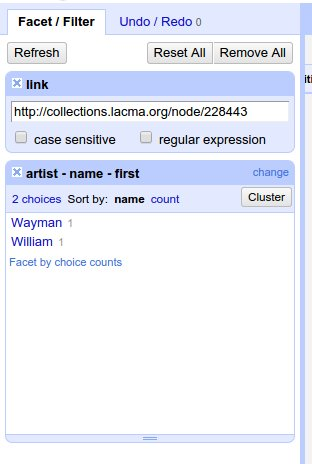
\includegraphics[width=0.34\textwidth]{artist2_after}}
        \caption{A filter on the artists of the particular painting returns rightly two entries}
        \end{figure}
        \pagebreak
        \subsection{bibliography}
        \begin{figure}[!ht]
        \centering
        \begin{subfigure}{0.8\textwidth}
        \centering
        \fbox{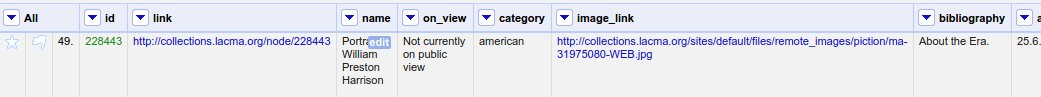
\includegraphics[width=0.95\textwidth]{bibliography_before1}}
        \caption{1st item of bibliography}
        \end{subfigure}
        \begin{subfigure}{0.8\textwidth}
        \centering
        \fbox{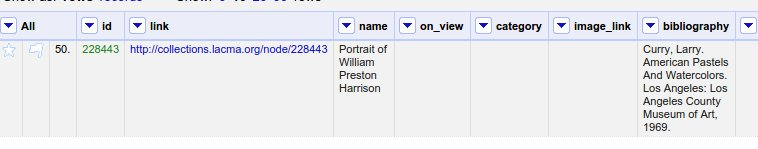
\includegraphics[width=0.95\textwidth]{bibliography_before2}}
        \caption{3rd item of bibliography}
        \end{subfigure}
        \begin{subfigure}{0.8\textwidth}
        \centering
        \fbox{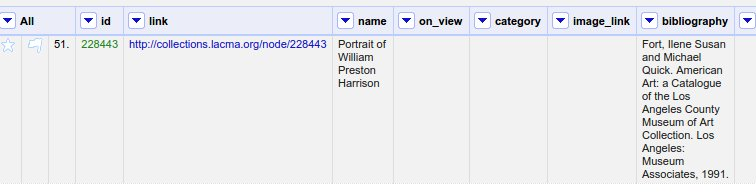
\includegraphics[width=0.95\textwidth]{bibliography_before3}}
        \caption{3rd item of bibliography}
        \end{subfigure}
        \caption{Before Cleaning}
        \end{figure}
        \begin{figure}[!ht]
        \centering
        \begin{subfigure}{0.8\textwidth}
        \centering
        \fbox{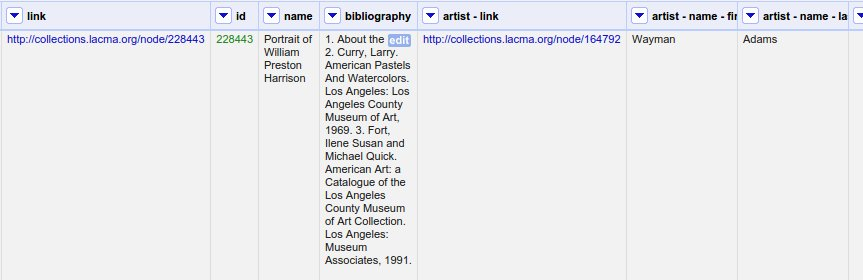
\includegraphics[width=0.95\textwidth]{bibliography_after1}}
        \caption{1st author's bibliography}
        \end{subfigure}
        \begin{subfigure}{0.8\textwidth}
        \centering
        \fbox{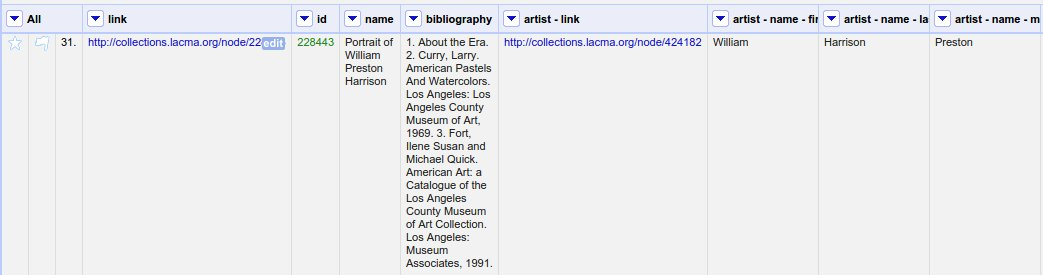
\includegraphics[width=0.95\textwidth]{bibliography_after2}}
        \caption{2nd author's bibliography}
        \end{subfigure}
        \caption{After Cleaning}
        \end{figure}
    \end{flushleft}
    
\end{homeworkProblem}

\end{document}